\section{Les équations de Serre}
\label{sec:Serre}
%% à reviser le math

\subsection{Le modèle}

\indent Les équations de Serre constituent un modèle qui décrit la propagation d'ondes fortement non linéaires dans des eaux peu profondes. En considérant un fond plat, ces équations s'écrivent sous la forme suivante, pour les variables $(h,u)$:

\begin{equation}
\label{eq:serrehu}
\begin{cases}
h_t + (hu)_x = 0 \\
u_t + uu_x + gh_x - \frac{1}{3h}\left(h^3 \left( u_{xt} + uu_{xx} - (u_x)^2  \right) \right)_x = 0
\end{cases}
\end{equation}

\noindent où $u = u(x,t)$, $h = h(x,t)$ et $g$ sont, respectivement, la vitesse horizontal moyennée au long de la profondeur, la profondeur de l'eau et l'accélération de la gravité. Cette formulation s'est basée sur \cite{CarterCienfuegos2011}.

\subsubsection{Les équations de Serre dans les variables $(h,hu)$}

\indent Afin de mettre en œuvre une méthode de \emph{splitting} pour la résolution numérique des équations de Serre (ainsi comme il est fait dans \cite{Bonneton2011} pour les équations de Green-Naghdi, qui sont la version en 2D de les équations de Serre), on va réécrire le système \eqref{eq:serrehu} dans les variables $(h,hu)$, afin d'avoir une formulation analogue à celle utilisé dans ce papier.

\indent On va utiliser les identités

\begin{equation*}
	(hu^2)_x = (huu)_x = (hu)_xu + huu_x
\end{equation*}

\noindent et, de la première équation de \eqref{eq:serrehu},

\begin{equation*}
	hu_t = (hu)_t - h_tu = (hu)_t +  (hu)_xu
\end{equation*}

\indent En multipliant la deuxième équation de \eqref{eq:serrehu} par $h$, on obtient

%\begin{equation}
%	\label{eq:serreTimesh}
%	\begin{aligned}
%		&& & hu_t + huu_x + ghh_x - \frac{1}{3}\left(h^3 \left( u_{xt} + uu_{xx} - (u_x)^2  \right) \right)_x = 0 \\
%		&& \implies & (hu)_t +  (hu)_xu + (hu^2)_x - (hu)_xu + ghh_x - \frac{1}{3}\left(h^3 \left( u_{xt} + (uu_x)_x - 2(u_x)^2  \right) \right)_x = 0  \\
%		&& \implies & (hu)_t +  (hu^2)_x  + ghh_x - \frac{1}{3}\left(h^3 \left( u_{xt} + (uu_x)_x - 2(u_x)^2  \right) \right)_x = 0 
%	\end{aligned}
%\end{equation}

\begin{equation}
	\label{eq:serreTimesh}
	\begin{aligned}
	(hu)_t +  (hu^2)_x  + ghh_x - \frac{1}{3}\left(h^3 \left( u_{xt} + (uu_x)_x - 2(u_x)^2  \right) \right)_x = 0 
	\end{aligned}
\end{equation}

\indent On remarque que

\begin{equation*}
	\begin{split}
	u_{xt} = \left(\frac{1}{h} (hu) \right)_{xt} = \left( -\frac{h_t}{h^2}(hu) + \frac{1}{h}(hu)_t  \right)_x = \left( -\frac{h_tu}{h} + \frac{1}{h}(hu)_t  \right)_x &= \\ \left( \frac{1}{h} ((hu)_xu) \right)_x  + \left( \frac{1}{h}(hu)_t  \right)_x &=0
	\end{split}
\end{equation*}

\noindent et

\begin{equation*}
	\begin{split}
	(uu_x)_x = \left(  \frac{1}{h} (huu_x) \right)_x = \left(  \frac{1}{h} ((hu^2)_x - (hu)_xu) \right)_x = \left( \frac{1}{h} (hu^2)_x \right)_x - \left( \frac{1}{h} (hu)_xu \right)_x
	\end{split}
\end{equation*}

\noindent alors, dans \eqref{eq:serreTimesh}, on obtient

\begin{equation*}
	(hu)_t  + (hu^2)_x + ghh_x - \frac{1}{3}\left[h^3 \left( \left( \frac{1}{h}(hu)_t  \right)_x  + \left( \frac{1}{h} (hu^2)_x \right)_x  - 2(u_x)^2  \right) \right]_x = 0
\end{equation*}

\indent Cette dernier équation peut être écrite sous la forme

\begin{equation*}
\begin{split}
	\left(\opIhT \right) (hu)_t + \left(\opIhT \right)(hu^2)_x + ghh_x + h\opQ_1(u) + \\ \left(\opIhT \right) (ghh_x) - \left(\opIhT \right) (ghh_x) = 0
\end{split}
\end{equation*}

\noindent où le terme $\left(\opIhT \right)(ghh_x)$ a été ajouté et soustrait pour avoir une formulation équivalente à de \cite{Bonneton2011}. Les opérateurs $\opT$ et $\opQ$, aussi définis par \cite{Bonneton2011}, sont donnés par

\begin{gather*}
	\opT(w) = -\frac{1}{3h}(h^3w_x)_x = -\frac{h^2}{3}w_{xx} - hh_xw_x \\
	\opQ(w) = \frac{2}{3h}(h^3(w_x)^2  )_x = \frac{4h^2}{3}(w_xw_{xx}) + 2hh_x(w_x)^2
\end{gather*}

\indent Ainsi, le système qu'on va résoudre est 

\begin{equation}
\label{eq:serrehhu}
\begin{cases}
h_t + (hu)_x = 0 \\
\begin{split}
(\opIhT) (hu)_t + (\opIhT)(hu^2)_x + ghh_x + h\opQ_1(u) + \\ \left(\opIhT \right) (ghh_x) - \left(\opIhT \right) (ghh_x) = 0
\end{split}
\end{cases}
\end{equation}


\subsection{Discrétisation}

\indent Comme on a fait au préalable pour la résolution numérique de l'équation de KdV, on met en oeuvre une méthode de \emph{splitting} pour résoudre numériquement les équations de Serre \eqref{eq:serrehhu} : le système d'équations \eqref{eq:serrehhu} est décomposé en deux parties, la première contenant les termes d'advection, et la deuxième, les dérivées d'ordre supérieur.

\indent Alors, la résolution numérique demande la résolution, dans chaque pas de temps $[t_n, t_{n+1}]$, du problème suivant :

\begin{equation}
	\label{eq:splitSerre1}
	\begin{cases}
		\th_t + \left(\th\tu\right)_x = 0 \\
		(\th\tu)_t + (\th\tu^2)_x + g\th\th_x = 0 
	\end{cases}	
\end{equation}

\begin{equation}
	\label{eq:splitSerre2}
	\begin{cases}
		\lh_t = 0 \\
		(\lh\lu)_t  -g\lh\lh_x + (\opIhT)^{-1}\left[ g\lh\lh_x + \lh\opQ_1(\lu) \right] = 0
	\end{cases}	
\end{equation}

\begin{equation*}
\begin{cases}
(h,u)(x,t_{n+1}) = (\lh,\lu)(x,t_{n+1})
\end{cases}
\end{equation*}

\indent En dénotant les systèmes \eqref{eq:splitSerre1} et  \eqref{eq:splitSerre2} par les opérateurs $T_a^{\Delta t}$ et $T_d^{\Delta t}$, respectivement, où le superindice indique que l'opérateur est appliqué sur un pas de temps  $\Delta t$, le problème peut s'écrire comme :

\begin{equation*}
(h,u)(x,t_{n+1}) = T_d^{\Delta t} \left( T_a^{\Delta t} \left((h,u)(x,t_n) \right) \right)
\end{equation*}

\indent Quelques variations de ce schéma de \emph{splitting} ont été également implémentés. Par exemple, en inversant l'ordre des opérateurs; ou encore la méthode connue comme \emph{"Strang splitting"}, où trois problèmes sont résolus dans chaque pas de temps :

\begin{equation*}
(h,u)(x,t_{n+1}) = T_a^{\frac{\Delta t}{2}} \left( T_d^{\Delta t} \left( T_a^{\frac{\Delta t}{2}} (h,u)(x,t_n) \right) \right)
\end{equation*}

\indent Dans las suite, le tilde et la barre supérieur seront supprimées pour clarifier la notation.

\subsubsection{Première système d'équations (pas d'advection)}

\indent La première partie des équations de Serre correspond au \emph{Non linear Shallow Water equations} (NSWE), qui peut être écrit comme une loi de conservation sous la forme

\begin{equation*}
	\boldsymbol{U}_t + \boldsymbol{F}(\boldsymbol{U})_x = 0
\end{equation*}

\noindent où

\begin{equation*}
	\boldsymbol{U} = \left(  \begin{array}{c} h \\ hu \end{array} \right), \qquad \boldsymbol{F}(\boldsymbol{U}) = \left(  \begin{array}{c} hu \\ hu^2 + \frac{1}{2}gh^2 \end{array} \right)
\end{equation*}

\indent Alors, on peut résoudre le première pas du \emph{splitting} en utilisant un schéma de volumes finies. La méthode implémentée utilise le solveur de Riemann approximée \emph{vfRoe-ncv} y une interpolation MUSCL d'ordre quatre sur chaque interface, ce qui réduit l'erreur de troncature et assure la non-négativité de la hauteur de l'eau. Par ailleurs, on a appliqué la méthode de reconstruction hydrostatique de deuxième ordre pour les termes source qui comprennent la topographie afin de préserver des états stationnaires de repos dans le cas où il y a de variabilité de la bathymétrie.

\indent Dans ce rapport, on se limite à cette brève description de la méthode de volumes finis utilisée, en considérant que, dans la division de tâches au sein de l'équipe, elle a été étudiée, codée et testée par José Galaz.


\subsubsection{Deuxième système d'équations (pas de dispersion)}

\indent Dans le deuxième système \eqref{eq:splitSerre2} des équations de Serre splittées, la profondeur d'eau $h$ est constante en temps, et par conséquent seulement la vitesse $u$ doit être mise à jour.  La résolution numérique proposée consiste en résoudre, à chaque pas de temps, le système linéaire

\begin{equation}
	\label{eq:systemhu}
	\left(\opIhT \right)^{-1}\left[ hh_x + h\opQ_1(u) \right]  = z \implies \left(\opIhT \right)z = hh_x + h\opQ_1(u)
\end{equation}

\indent Le côté à gauche de \eqref{eq:systemhu} s'écrit

%\begin{equation*}
%\begin{aligned}
%	 \left(\opIhT\right)z  & =  z - \frac{h^3}{3}\left( \frac{1}{h} z\right)_{xx} - h^2h_x\left( \frac{1}{h} z\right)_x  = \\
%						  & = z - \frac{h^3}{3}\left[ \left( 2\frac{(h_x)^2}{h^3} - \frac{h_{xx}}{h^2} \right)z - 2\frac{h_x}{h^2}z_x + \frac{z_{xx}}{h}	\right] - h^2h_x\left[ -\frac{h_x}{h^2}z + \frac{z_x}{h}\right] = \\
%						  &  = \left( 1 + \frac{1}{3}(h_x)^2 + \frac{1}{3}hh_{xx}\right)z - \left(\frac{1}{3}hh_x\right)z_x - \left(\frac{1}{3}h^2\right)z_{xx}
%\end{aligned}
%\end{equation*}

\begin{equation*}
\begin{aligned}
	 \left(\opIhT\right)z  & =  z - \frac{h^3}{3}\left( \frac{1}{h} z\right)_{xx} - h^2h_x\left( \frac{1}{h} z\right)_x  = \\
						  &  = \left( 1 + \frac{1}{3}(h_x)^2 + \frac{1}{3}hh_{xx}\right)z - \left(\frac{1}{3}hh_x\right)z_x - \left(\frac{1}{3}h^2\right)z_{xx}
\end{aligned}
\end{equation*}

\indent En utilisant des différences finies d'ordre quatre pour discrétiser les dérivées spatiales de $z$, on résoudre, pour chaque $i = 1,...,N-1$ dans le pas de temps $t_n$ :

\begin{equation*}
	\begin{split}
	 \left( 1 + \frac{1}{3}((h_x)_i^n)^2 + \frac{1}{3}h_i^n (h_{xx})_i^n + \frac{1}{\Delta x^2}\frac{5}{6}(h_i^n)^2\right)z_i^n + \\
	   \frac{1}{3}\left( -\frac{2}{3}\frac{h_i^n(h_x)_i^n}{\Delta x} - \frac{4}{3}\frac{(h_i^n)^2}{\Delta x^2} \right)z_{i+1}^n +  \frac{1}{3}\left( \frac{2}{3}\frac{h_i^n(h_x)_i^n}{\Delta x} - \frac{4}{3}\frac{(h_i^n)^2}{\Delta x^2} \right)z_{i-1}^n  + \\
	   \frac{1}{36}\left( \frac{h_i^n(h_x)_i^n}{\Delta x} + \frac{4}{3}\frac{(h_i^n)^2}{\Delta x^2} \right)z_{i+2}^n + \frac{1}{36}\left( -\frac{h_i^n(h_x)_i^n}{\Delta x} + \frac{4}{3}\frac{(h_i^n)^2}{\Delta x^2} \right)z_{i-2}^n  = \\
	    h_i^n(h_x)_{i}^n  + h_i^n(\opQ_1(u))_i^n
	\end{split}
\end{equation*}

\indent Finalement, pour chaque $i=1,...N-1$, las solution est mise à jour en temps selon l'expression 

\begin{equation*}
(hu)_i^{n+1} = (hu)_i^n + \Delta t \left(gh_i^n(h_x)_i^n - z_i^n \right)
\end{equation*}

\subsection{Tests numériques}

\subsubsection{Description de la solution initiale}

\indent Afin de valider l'implémentation des équations de Serre, on les a résolues en utilisant son solution analytique comme solution initiale. D'après \cite{CarterCienfuegos2011}, les équations de Serre admettent la famille de solutions périodiques suivante : 

\begin{equation*}
    h(x,t) = a_0 + a_1 dn^2(\kappa(x-ct),k), \qquad
    u(x,t) = c\left( 1 - \frac{h_0}{h(x,t)}\right)
\end{equation*}

\begin{equation*}
    \kappa = \frac{\sqrt{3a_1}}{2\sqrt{a_0(a_0+a_1)(a_0+(1-k^2)a_1)}}, \qquad
    c = \frac{\sqrt{g a_0(a_0+a_1)(a_0+(1-k^2)a_1)}}{h_0}
\end{equation*}

\noindent avec $k\in(0,1)$, $a_0>0$, $a_1>0$ et $dn(\cdot,k)$ une fonction elliptique de Jacobi de module $k$.

\indent La relation entre la longueur d'onde $\lambda$ et $k\in(0,1)$ est $$\lambda = \frac{2K(k)}{\kappa}$$ et la profondeur moyenne de l'eau, $h_0$, est calculée à partir de $$h_0 = \frac{1}{\lambda}\int_{0}^\lambda h(x,t)dx = a_0 + a_1 \frac{E(k)}{K(k)}$$

\noindent où $K(k)$ et $E(k)$ sont des intégrales elliptiques complètes de premier et deuxième types. 

\indent La limite pour $k\to0^+$ est le niveau constant de l'eau $a_0+a_1$ en équilibre. Si $k\to1^-$, $(h,u)$ converge vers la solution de Rayleigh (onde solitaire). On a testé aussi ce dernier cas, dans lequel la solution est décrite par \cite{CarterCienfuegos2011}

\begin{equation*}
    h(x,t) = a_0 + a_1 sech^2(\kappa(x-ct),k), \qquad
    u(x,t) = c\left( 1 - \frac{a_0}{h(x,t)}\right)
\end{equation*}

\begin{equation*}
    \kappa = \frac{\sqrt{3a_1}}{2\sqrt{a_0(a_0+a_1)}}, \qquad
    c = \sqrt{g a_0(a_0+a_1)}
\end{equation*}

\indent Les expressions para la longueur d'onde $\lambda$ et la profondeur moyenne de l'eau $h_0$ sont les mêmes que pour le cas général de la solution cnoïdale.

\subsubsection{Résultats}

\indent Afin d'observer les effets nonlinéaires et dispersives dans le modèle, on a résolu les équations de Serre et les équations nonlinéaires de \emph{Shallow Water} (NSWE). Ce dernier système d'équations est en fait le premier pas du schéma de \emph{splitting} proposé. Les figures \ref{fig:cnoidalh} et \ref{fig:cnoidalu} montrent l'évolution de $(h,u)$ pour la solution cnoïdale, et les figures  \ref{fig:solitaryh} et \ref{fig:solitaryu} le montrent dans le cas de la solution solitaire. 

\begin{figure}[h!]
	\begin{subfigure}{.3\linewidth}
		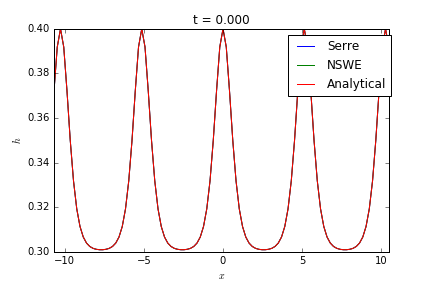
\includegraphics[scale=.3]{figures/Serre/4x4cnoidal1h.png}	
	\end{subfigure}
	\begin{subfigure}{.3\linewidth}
		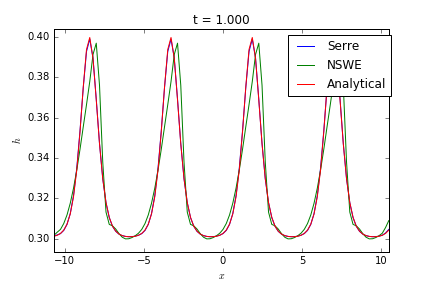
\includegraphics[scale=.3]{figures/Serre/4x4cnoidal2h.png}	
	\end{subfigure}
	\begin{subfigure}{.3\linewidth}
		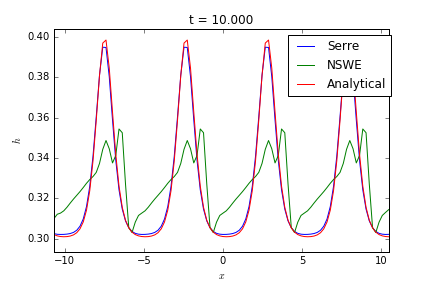
\includegraphics[scale=.3]{figures/Serre/4x4cnoidal3h.png}	
	\end{subfigure}
	\caption{Évolution de $h$ pour la solution cnoïdale des équations de Serre. Comparaison entre la solution analytique (en rouge) et les solutions donnés par les modèles de Serre (en bleu) et les NSWE (en vert). \label{fig:cnoidalh}}
\end{figure}

\begin{figure}[h!]
	\begin{subfigure}{.3\linewidth}
		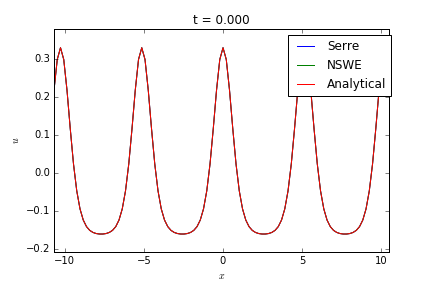
\includegraphics[scale=.3]{figures/Serre/4x4cnoidal1u.png}	
	\end{subfigure}
	\begin{subfigure}{.3\linewidth}
		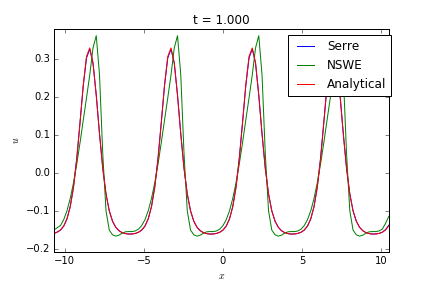
\includegraphics[scale=.3]{figures/Serre/4x4cnoidal2u.png}	
	\end{subfigure}
	\begin{subfigure}{.3\linewidth}
		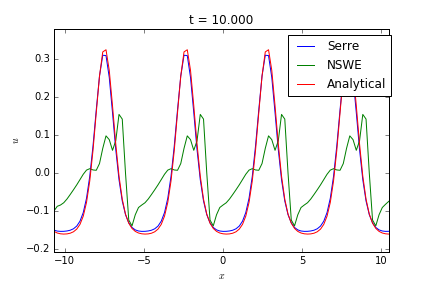
\includegraphics[scale=.3]{figures/Serre/4x4cnoidal3u.png}	
	\end{subfigure}
	\caption{Évolution de $u$ pour la solution cnoïdale des équations de Serre. Comparaison entre la solution analytique (en rouge) et les solutions donnés par les modèles de Serre (en bleu) et les NSWE (en vert).  \label{fig:cnoidalu}}
\end{figure}

\begin{figure}[h!]
	\begin{subfigure}{.3\linewidth}
		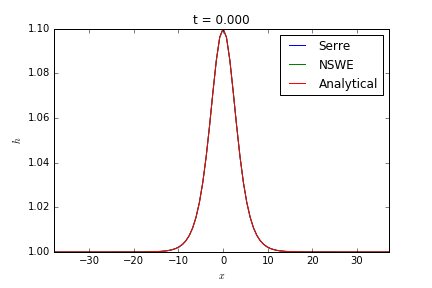
\includegraphics[scale=.3]{figures/Serre/4x4solitary1h.png}	
	\end{subfigure}
	\begin{subfigure}{.3\linewidth}
		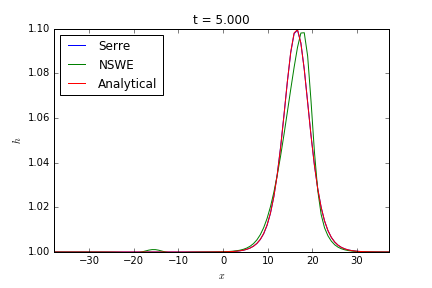
\includegraphics[scale=.3]{figures/Serre/4x4solitary2h.png}	
	\end{subfigure}
	\begin{subfigure}{.3\linewidth}
		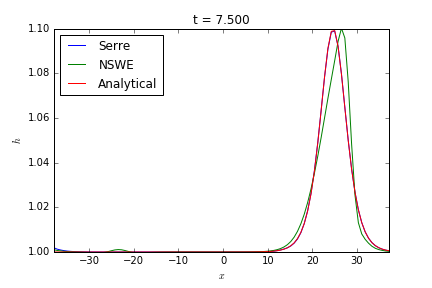
\includegraphics[scale=.3]{figures/Serre/4x4solitary3h.png}	
	\end{subfigure}
	\caption{Évolution de $h$ pour la solution solitaire des équations de Serre. Comparaison entre la solution analytique (en rouge) et les solutions donnés par les modèles de Serre (en bleu) et les NSWE (en vert). \label{fig:solitaryh}}
\end{figure}

\begin{figure}[h!]
	\begin{subfigure}{.3\linewidth}
		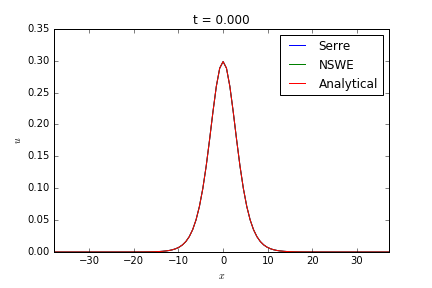
\includegraphics[scale=.3]{figures/Serre/4x4solitary1u.png}	
	\end{subfigure}
	\begin{subfigure}{.3\linewidth}
		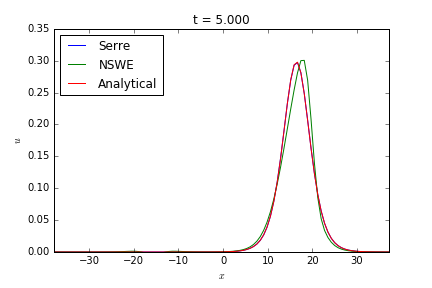
\includegraphics[scale=.3]{figures/Serre/4x4solitary2u.png}	
	\end{subfigure}
	\begin{subfigure}{.3\linewidth}
		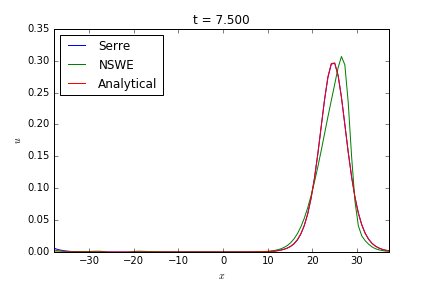
\includegraphics[scale=.3]{figures/Serre/4x4solitary3u.png}	
	\end{subfigure}
	\caption{Évolution de $u$ pour la solution solitaire des équations de Serre. Comparaison entre la solution analytique (en rouge) et les solutions donnés par les modèles de Serre (en bleu) et les NSWE (en vert).  \label{fig:solitaryu}}
\end{figure}

\indent On peut observer très clairement les effets du pas de dispersion sur la solution donnée par les NSWE. Le premier pas des équations de Serre splittées cause la formation de chocs. Par ailleurs, comme le schéma de volumes finis implémenté n'utilise pas des limiteurs, les discontinuités ne sont pas bien traitées, ce qui provoque les grandes déformations de la solution dans des instants plus avancées, comme montrent les dernières images dans les figures \ref{fig:cnoidalh} et \ref{fig:cnoidalu}. En revanche, dans la résolution des équations de Serre, le pas de dispersion fait une "correction" de la formation du choc, et la forme de la solution analytique est préservée.

\indent Ainsi, ces exemples numériques valident notre implémentation des équations de Serre. On remarque également que, aussi comme la forme, l'amplitude de la solution est bien préservée, avec une petite réduction. En fait, cet résultat a été obtenu seulement avec le schéma de volumes finies d'ordre 4. Au début, on a implémenté des schémas d'ordre 1 et 2, avec lesquels la réduction de l'amplitude était beaucoup plus importante (malgré la préservation de la forme), comme montre, à titre d'exemple, la figure \ref{fig:cnoidalhOrdre2}:

\begin{figure}[h!]
	\begin{subfigure}{.3\linewidth}
		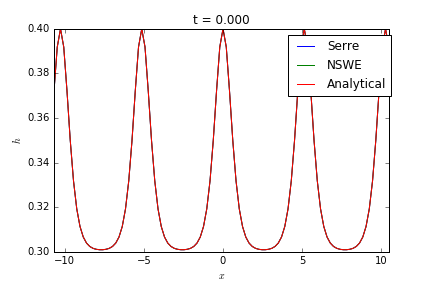
\includegraphics[scale=.3]{figures/Serre/cnoidal1h.png}	
	\end{subfigure}
	\begin{subfigure}{.3\linewidth}
		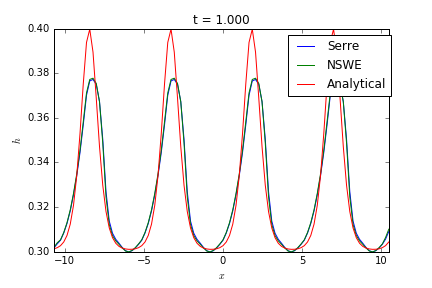
\includegraphics[scale=.3]{figures/Serre/cnoidal2h.png}	
	\end{subfigure}
	\begin{subfigure}{.3\linewidth}
		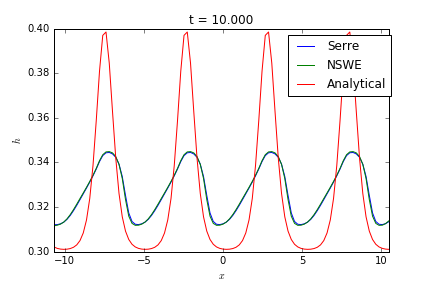
\includegraphics[scale=.3]{figures/Serre/cnoidal3h.png}	
	\end{subfigure}
	\caption{Évolution de $h$ pour la solution cnoïdale des équations de Serre. Comparaison entre la solution analytique (en rouge) et les solutions donnés par les modèles de Serre (en bleu) et les NSWE (en vert), avec une méthode de volumes finies d'ordre 2. \label{fig:cnoidalhOrdre2}}
\end{figure}